\section{Simulation}
\label{sec:simulation}

\subsection{Collapsed workflow}
\ididthis{Ettore Ricci, Paolo Palumbo, Francesco Boldrini}

\begin{figure}[H]
\centering
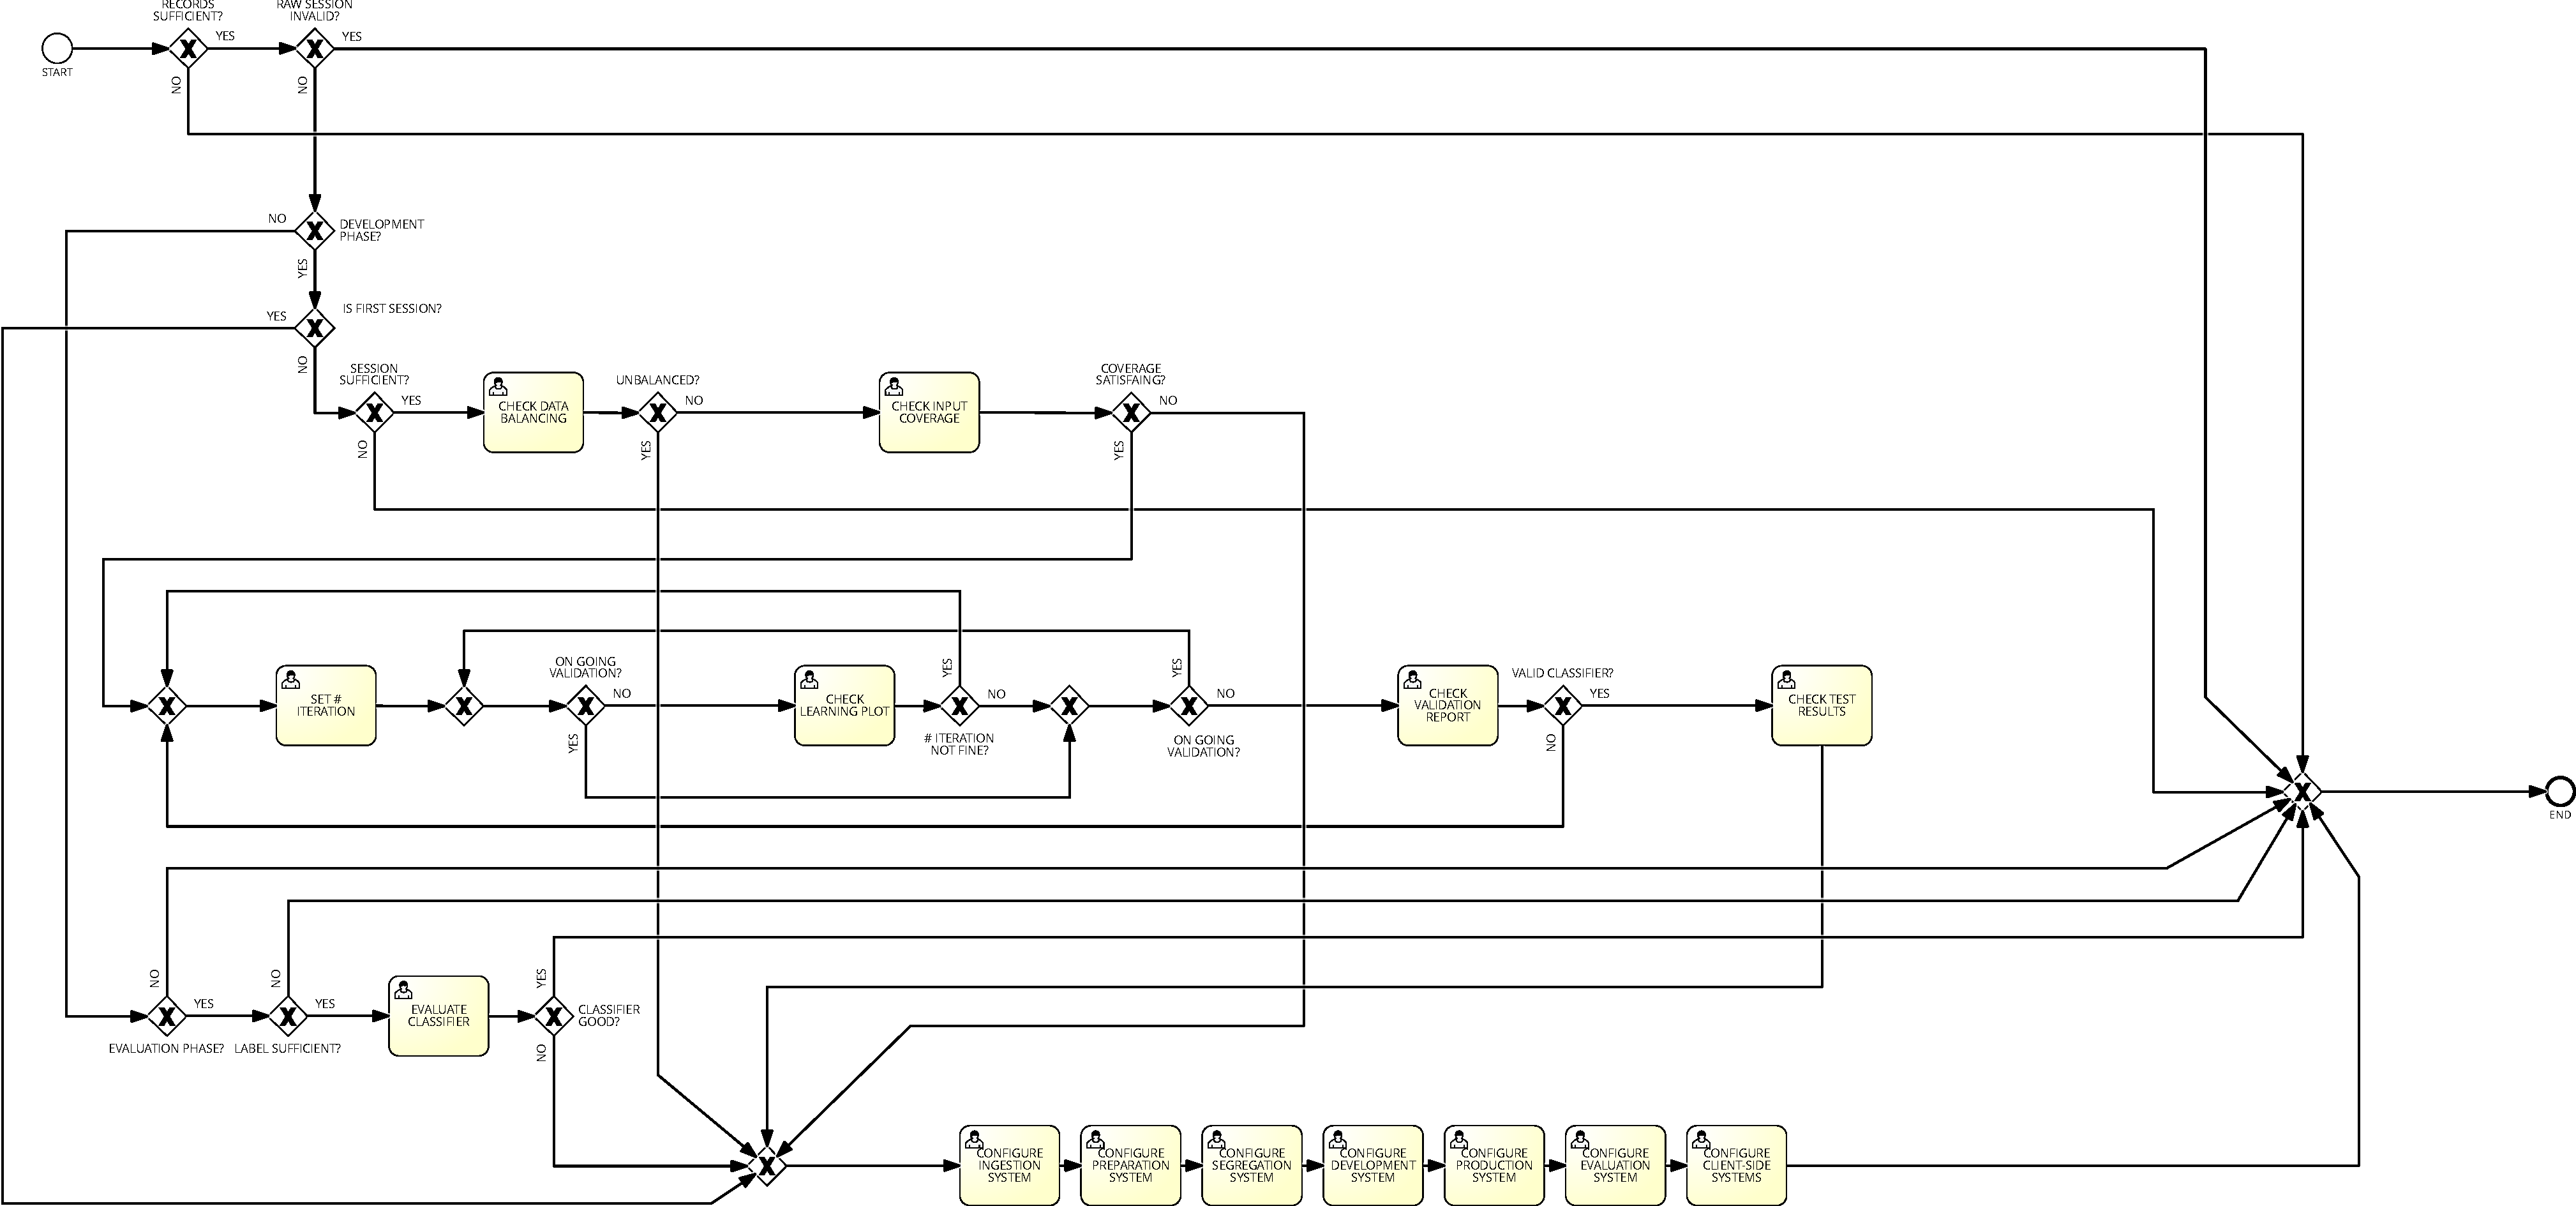
\includegraphics[width=1\textwidth]{figures/Collapsed Workflow SIM.pdf}
\caption{Collapsed workflow}
\label{fig:collapsed_workflow}
\end{figure}

\subsection{AS-IS Simulation}
\label{sec:as_is_simulation}
\ididthis{Francesco Boldrini, Zahra Omrani}

NB: we set the total number of initial process instances to 6852,
as with our assumptions for the two
initial gates, where we discard 10\% of the sessions twice, we need 6852 sessions to start, to work with
the documentation's assumptions of the 5550 good sessions for all phases altogether.

\begin{figure}[H]
    \centering
    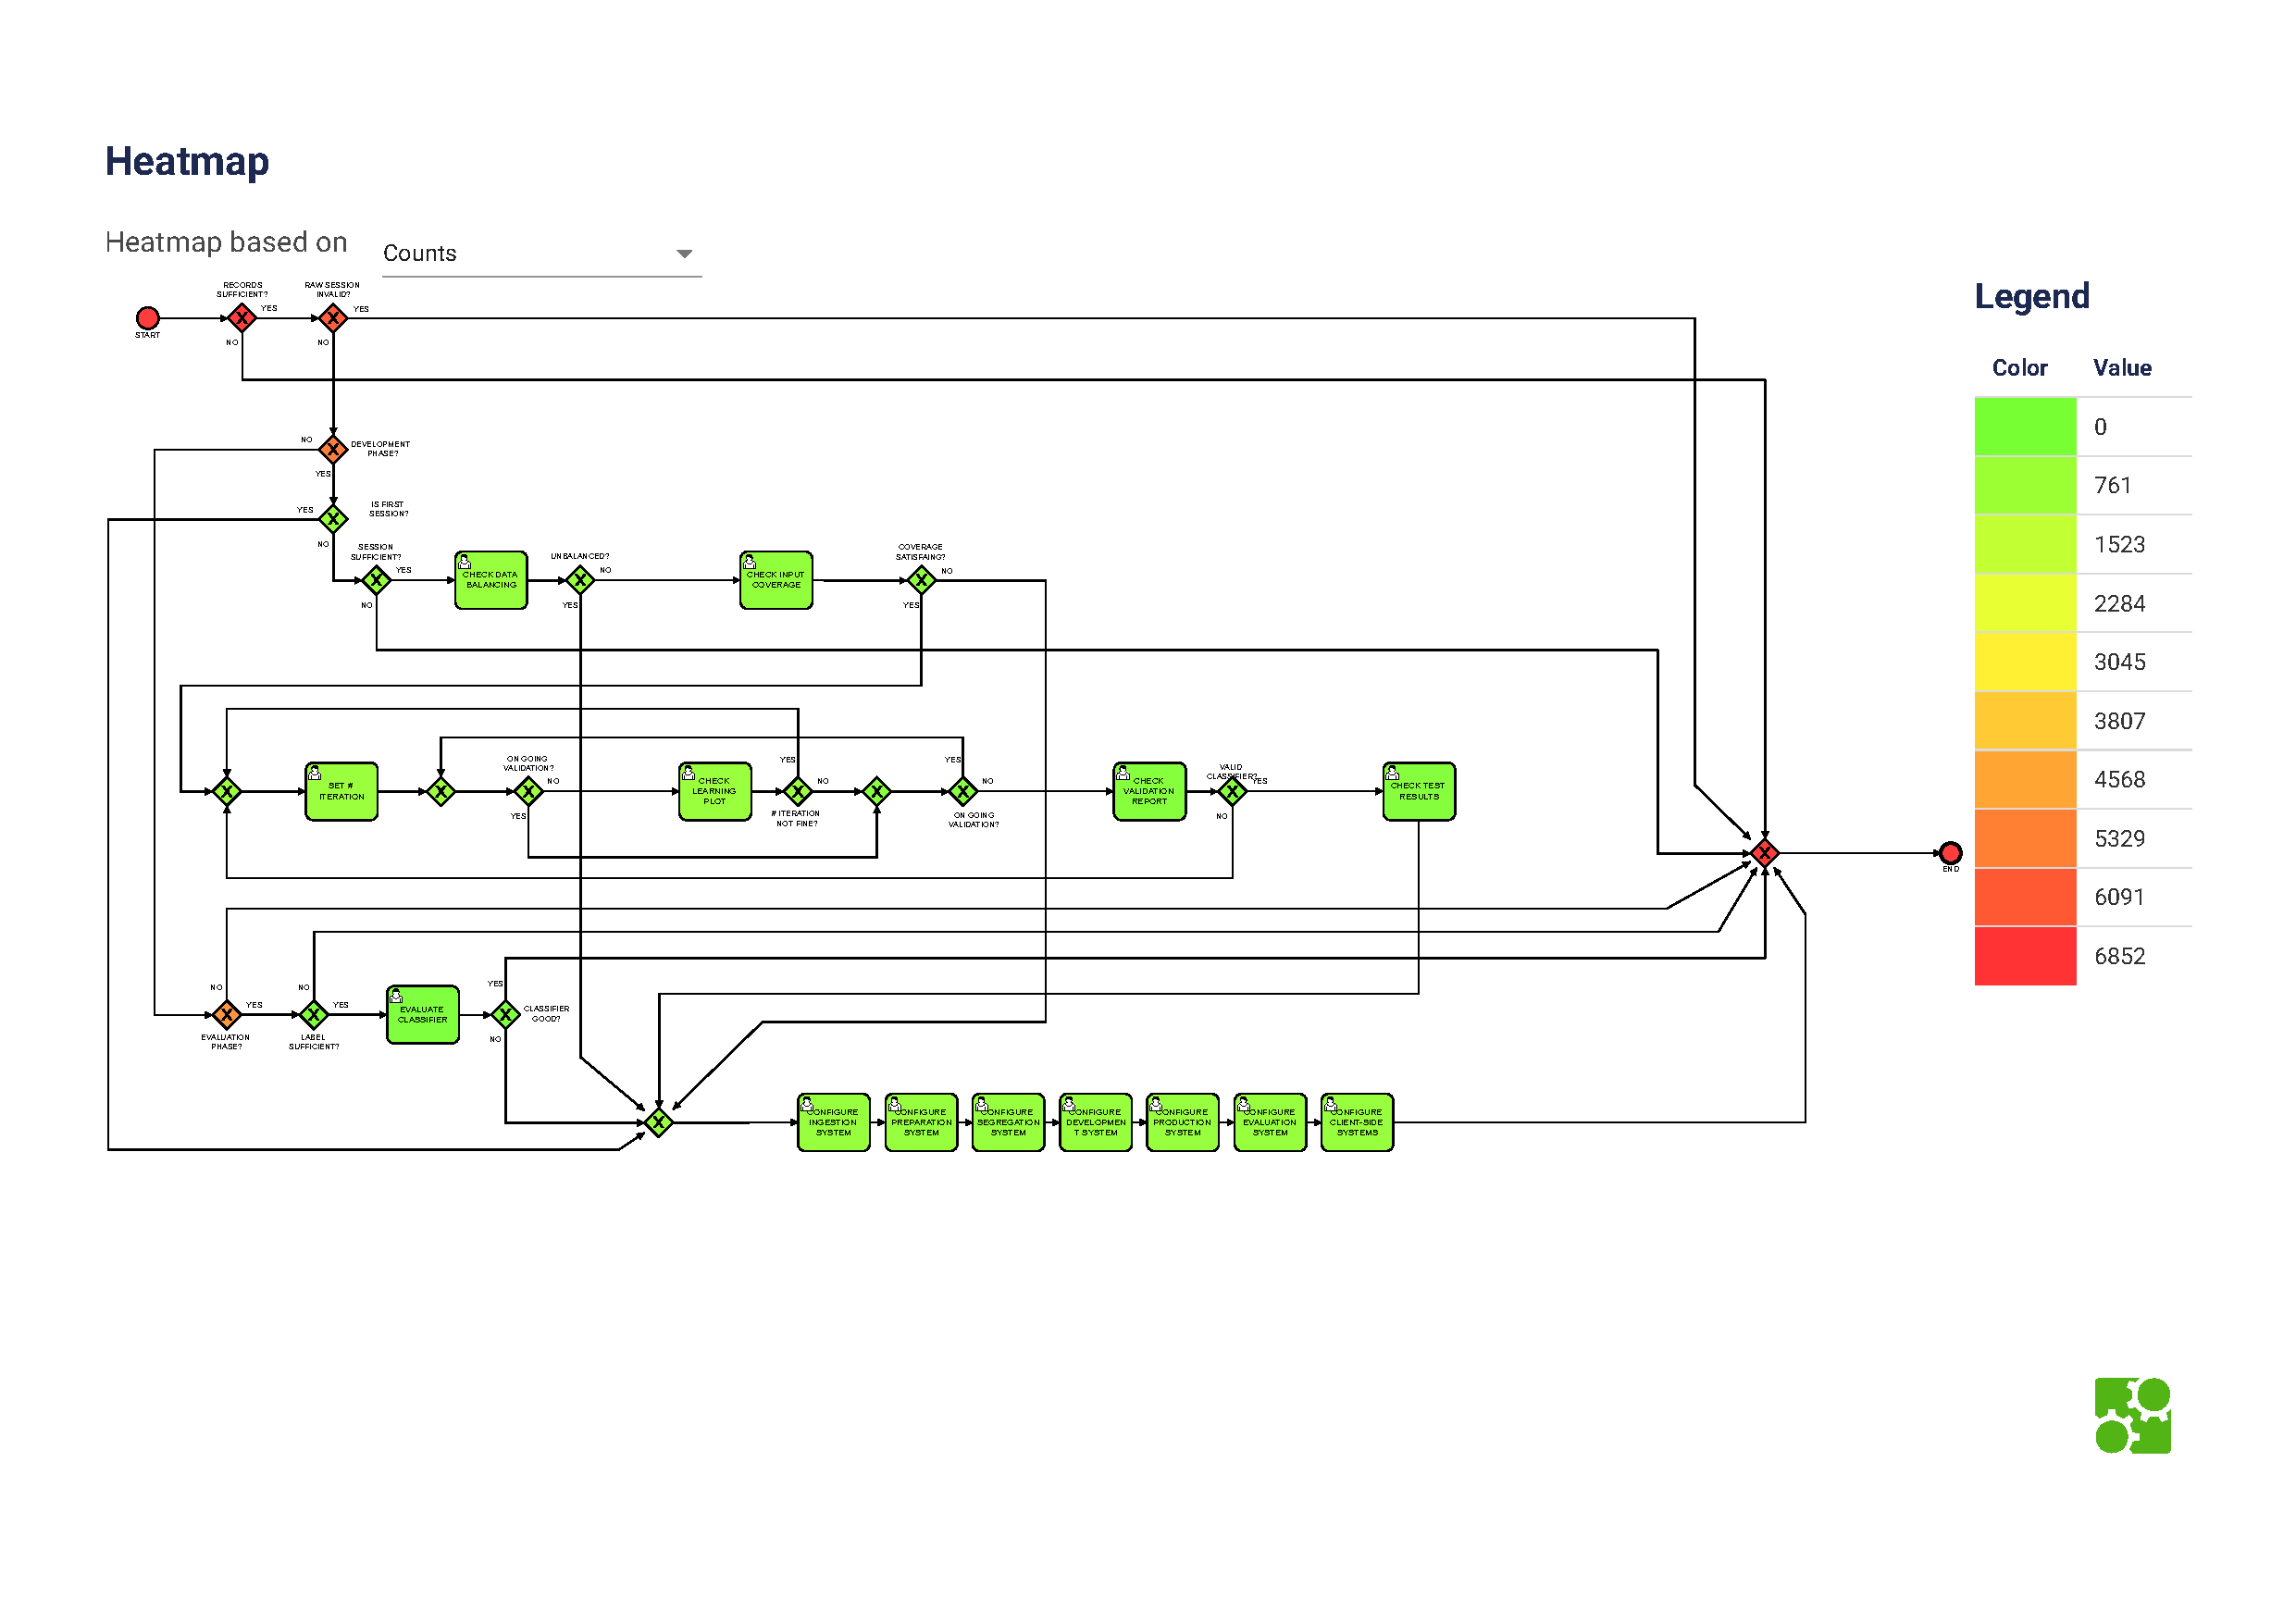
\includegraphics[width=0.87\textwidth]{figures/AS-IS heatmap_counts.pdf}
    \caption{AS-IS Heatmap of the counts of the parameters}
    \label{fig:as_is_heatmap_counts}
\end{figure}

\begin{figure}[H]
    \centering
    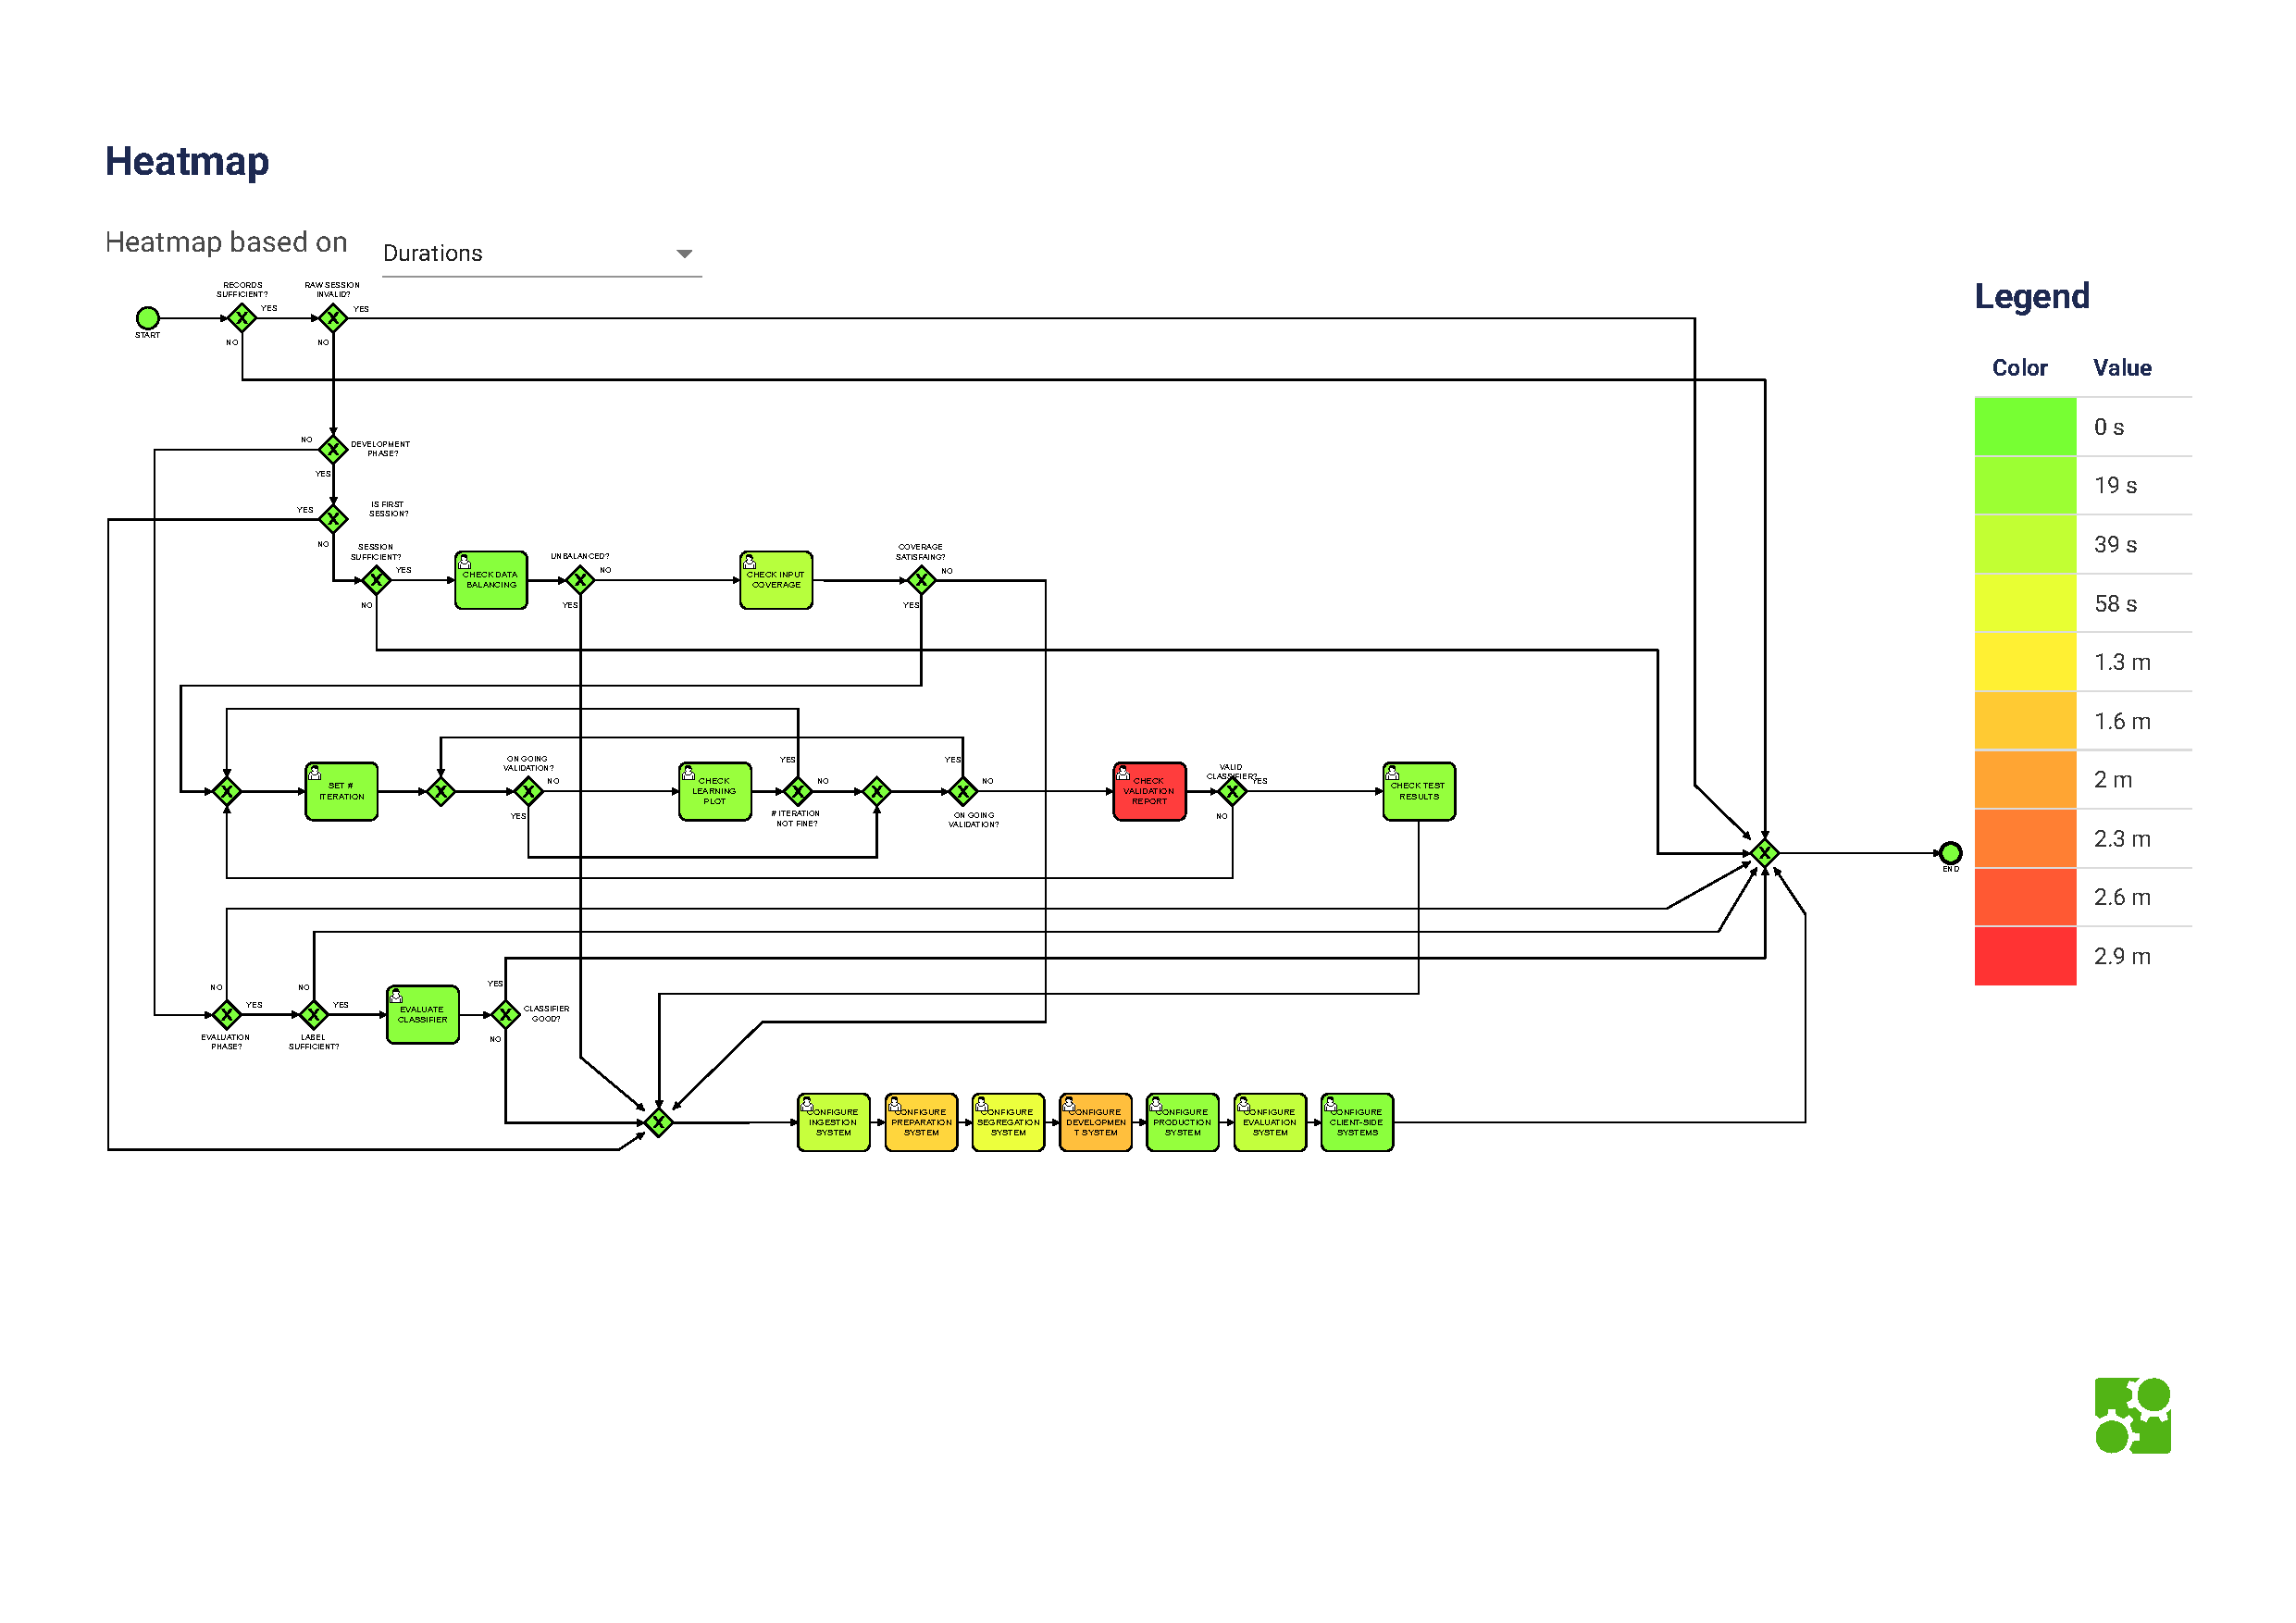
\includegraphics[width=0.87\textwidth]{figures/AS-IS heatmap_durations.pdf}
    \caption{AS-IS Heatmap of the time spent in each passage [Durations]}
    \label{fig:as_is_heatmap_durations}
\end{figure}

\begin{figure}[H]
    \centering
    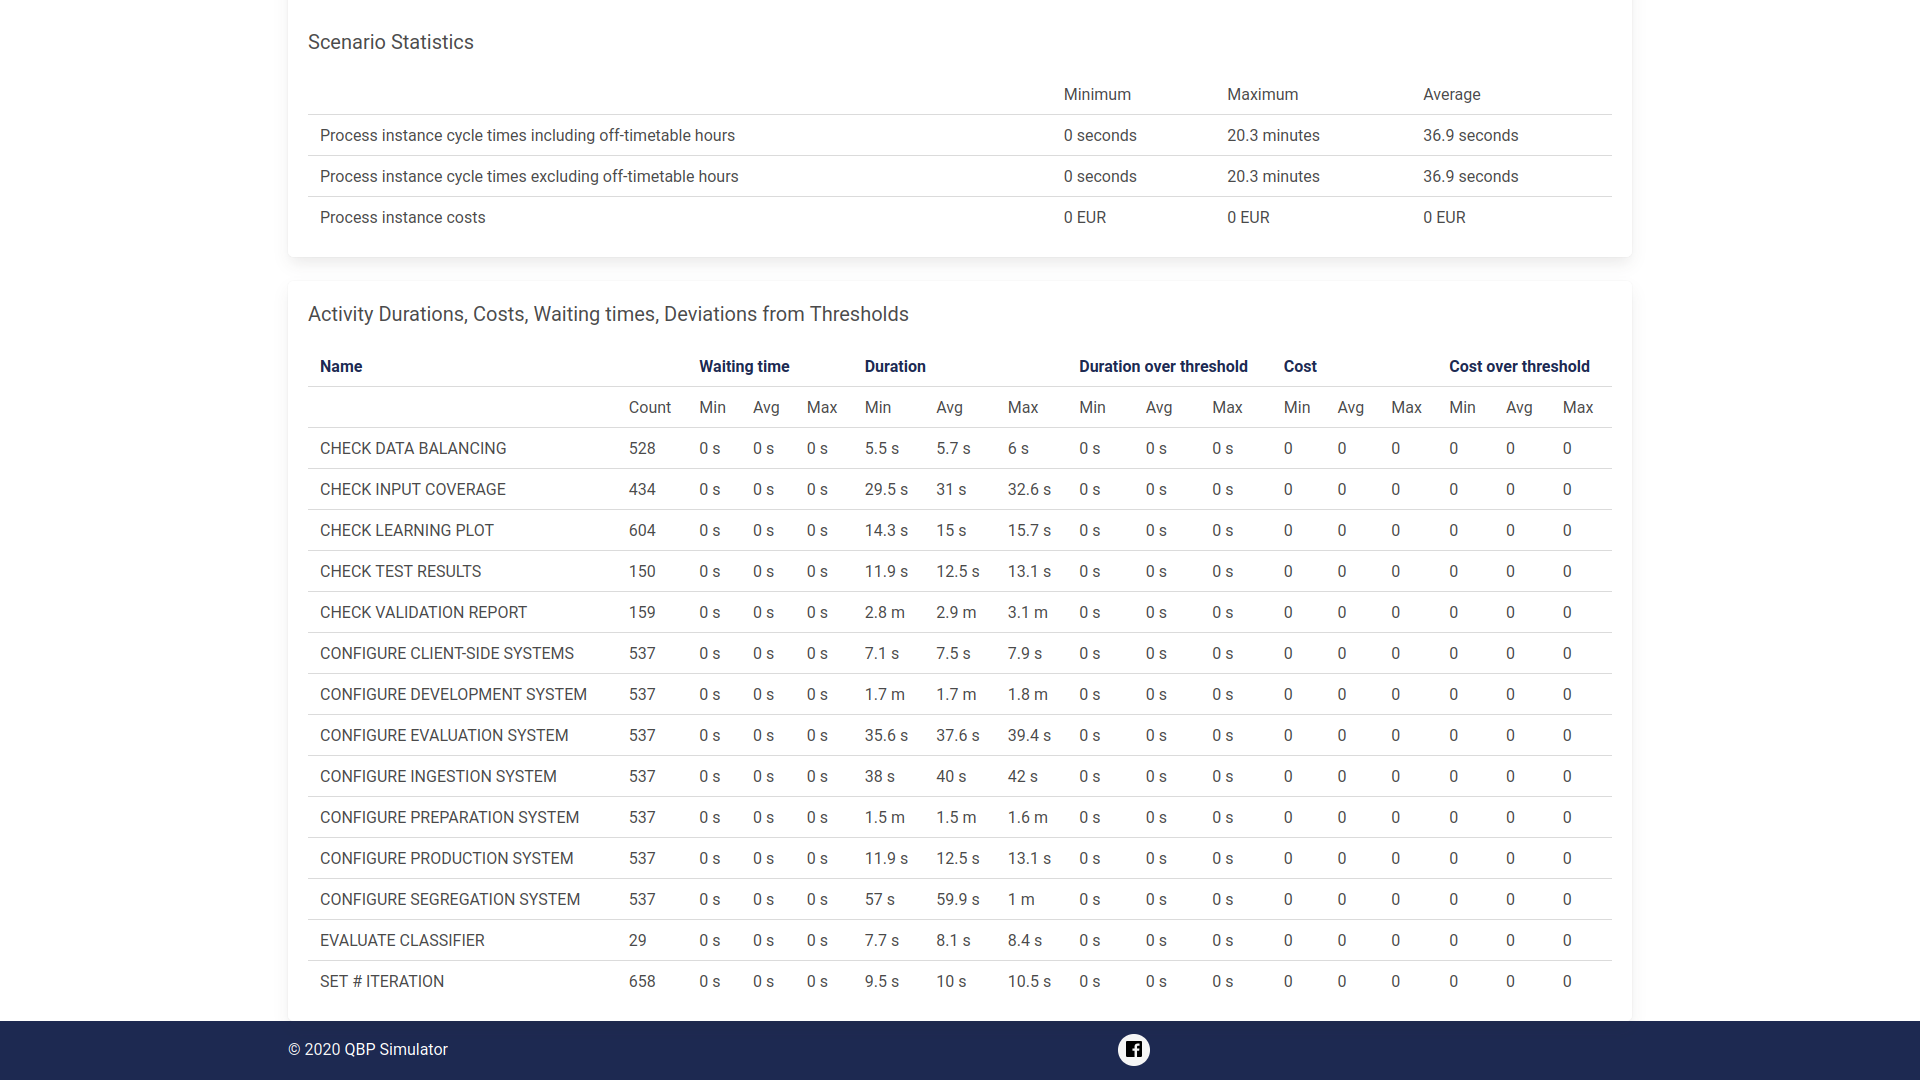
\includegraphics[width=1\textwidth]{figures/AS-IS Simulation Results.png}
    \caption{AS-IS Simulation Results}
    \label{fig:as_is_simulation_results}
\end{figure}

\begin{figure}[H]
    \centering
    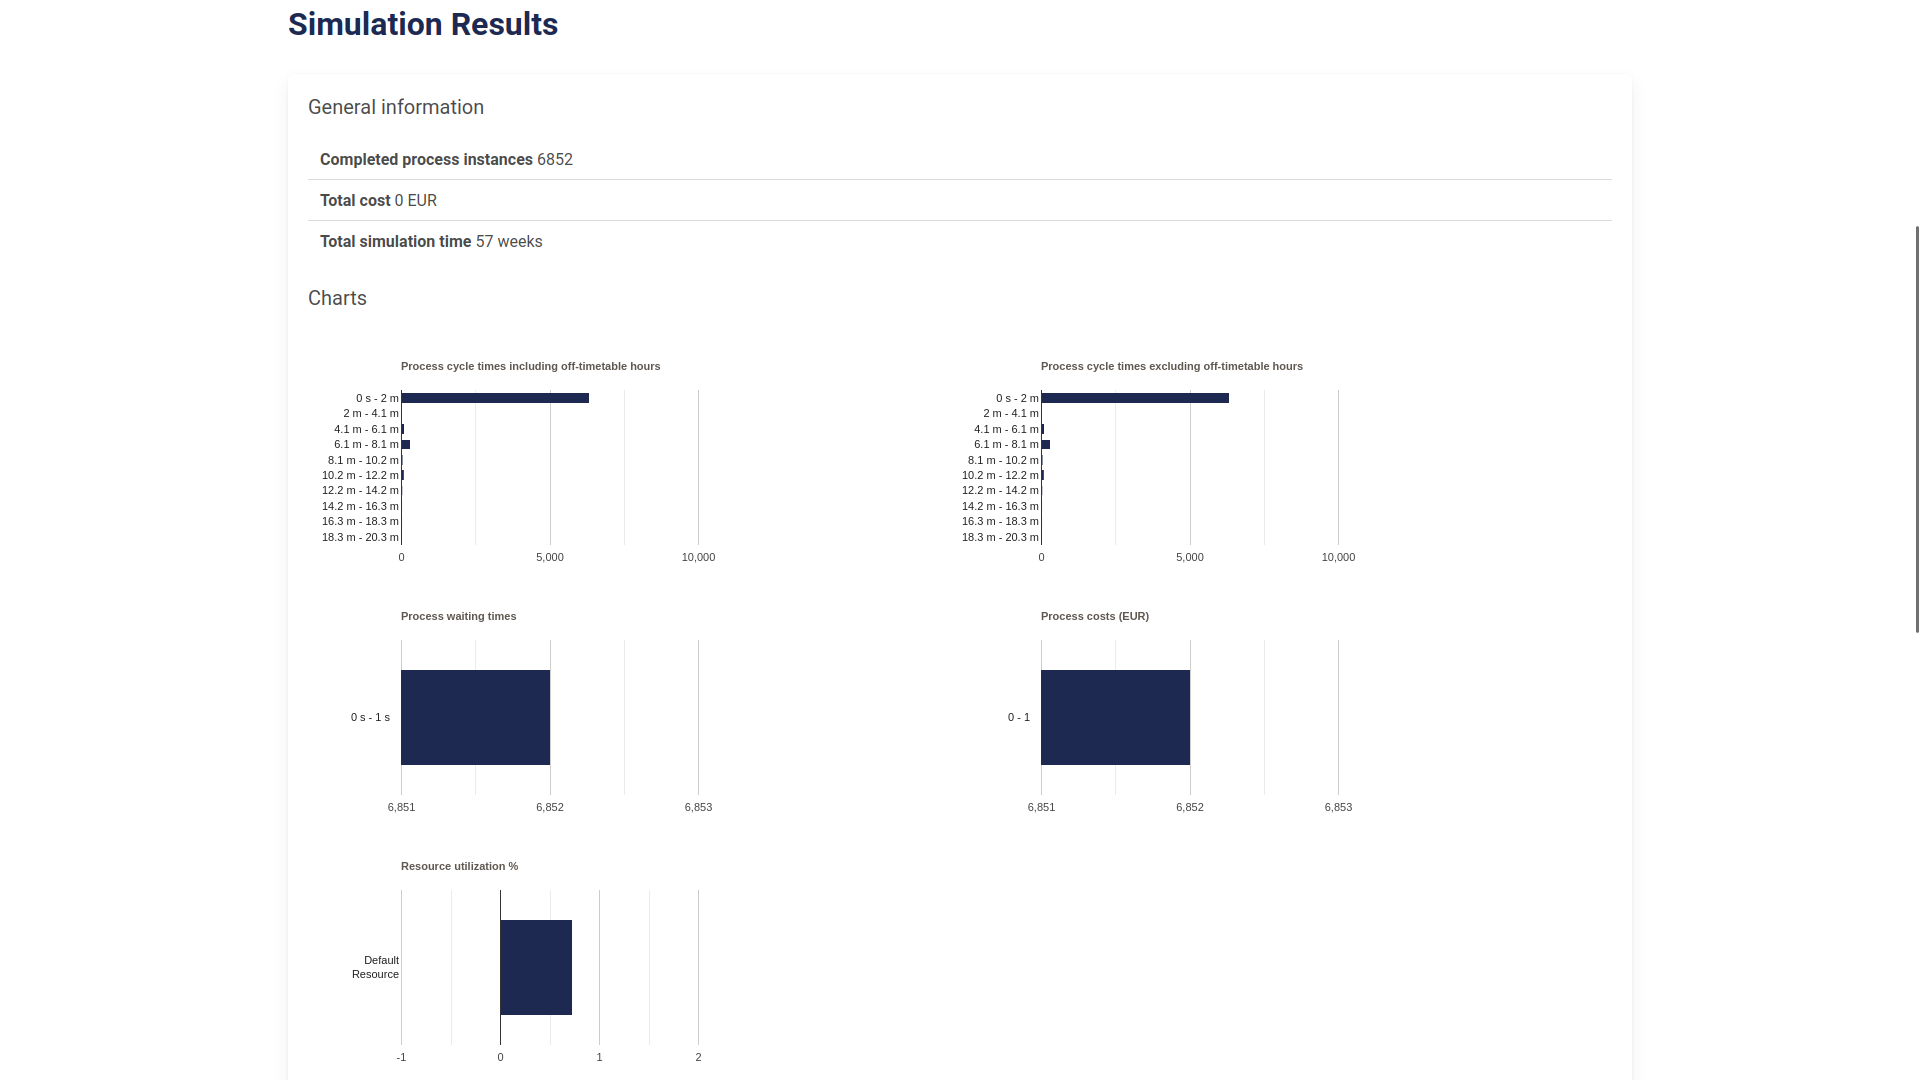
\includegraphics[width=1\textwidth]{figures/AS-IS Scenario Statistics.png}
    \caption{AS-IS Scenario Statistics}
    \label{fig:as_is_scenario_Statistics}
\end{figure}

\begin{table}[H]
    \centering
    \begin{tabularx}{\textwidth}{|X|c|l|}
    \hline
    \textbf{Parameter} & \textbf{\% of the Gate} & \textbf{Motivation} \\
    \hline
     \# Iteration not fine? & 20\% & According to the assumptions of the \\
     & & documentation, we set the \% of iters \\
     & & that are not fine to 20\% \\
    \hline
    Classifier Good? & 86\% & According to the assumptions of the \\
     & & docs, classifiers are good 86 of the time \\
    \hline
    Coverage satisfying? & 33\% & According to the assumptions of the \\
     & & docs, coverage is satisfying 33\% of the time \\
    \hline
    Development Phase? & 9\% & In this gate, out of 5550, 500 are \\
     & & in the development phase \\
    \hline
    Is First Session? & 1\% & In this gate, out of 500, 1 is 
    \\ & & in the first session, but the gate
    \\ & & won't load less than 1\% on BIMP 
    \\
    \hline
    Labels sufficient? & 71\% & Given 5550 good sessions, and 
    \\ & & assuming that those will yields
    \\ & & 5 proper classifiers, given the 
    \\ & & probabilities at the preceding 
    \\ & & gates and the rounding because of 
    \\ & & necessity of the gate to have at 
    \\ & & least 1\% as value, we 
    \\ & & need to have 71\% of the sessions 
    \\ & & to have sufficient labels to respect 
    \\ & & the documentation's assumptions.
    \\
    \hline
    On going Validation? & 90\% & We set validation to 90\% as most
    \\ & & of the times this step involves the
    \\ & & autonomous systems and not humans \\
    \hline
    Raw session Invalid? & 10\% & We assume that 90\% of the times
    \\ & & the raw session is valid.\\
    \hline
    Records Sufficient? & 90\% & We assume that 90\% of the times
    \\ & & the records are sufficient.\\
    \hline
    Session Sufficient? & 99\% & We set sessions sufficient to 99\% as
    \\ & & with the document's assumptions, we 
    \\ & & would need roughly 545 sessions to 
    \\ & & have 5 final good classifiers and here
    \\ & &  we already start with 500, which is
    \\ & & already lower than what we would need.\\
    \hline
    Unbalanced? & 20\% & The documentation assumes that
    \\ & &  20\% of the classes are balanced\\
    \hline
    Valid Classifier? & 95\% & The documentation assumes that
    \\ & &  95\% of the classifiers are valid\\
    \hline

\end{tabularx}
\end{table}


\subsection{Modeling the TO-BE Process}
\label{sec:modeling_to_be_processing}
\ididthis{Francesco Boldrini, Zahra Omrani}

In the context of our application, "Emotion Based Music Selection", we suppose that during the initial configuration phase, we acquire the data through the ECG sensors and the user's schedules, currently playing music and other relevant informations.

This data could be processed by a research center through data-mining approaches: this would mean simplifying the process and making it more efficient, as we could use existing similar classifiers to initialize ours, rather than starting from scratch.

In fact similar networks and classifiers may work well with similar parameters over similar tasks.

For each category it is possible to define some improvement(s):

1. Hand-Off level Improvement(s): Re-use sessions from similar networks in the same category, rather than collecting other sessions.

2. Service Level Improvement(s): Use hyperparameters from similar networks in the same category, rather than starting from scratch.

3. Task Level Improvement(s): Reduce the cognitive effort necessary for the configurations, by starting from default parameters obtained from other similar networks, rather than starting from scratch.


\subsubsection{Hand-Off level Improvement(s)}
\label{subsec:hand_off_level_improvements}
\ididthis{Francesco Boldrini, Zahra Omrani}


\begin{figure}[H]
    \centering
    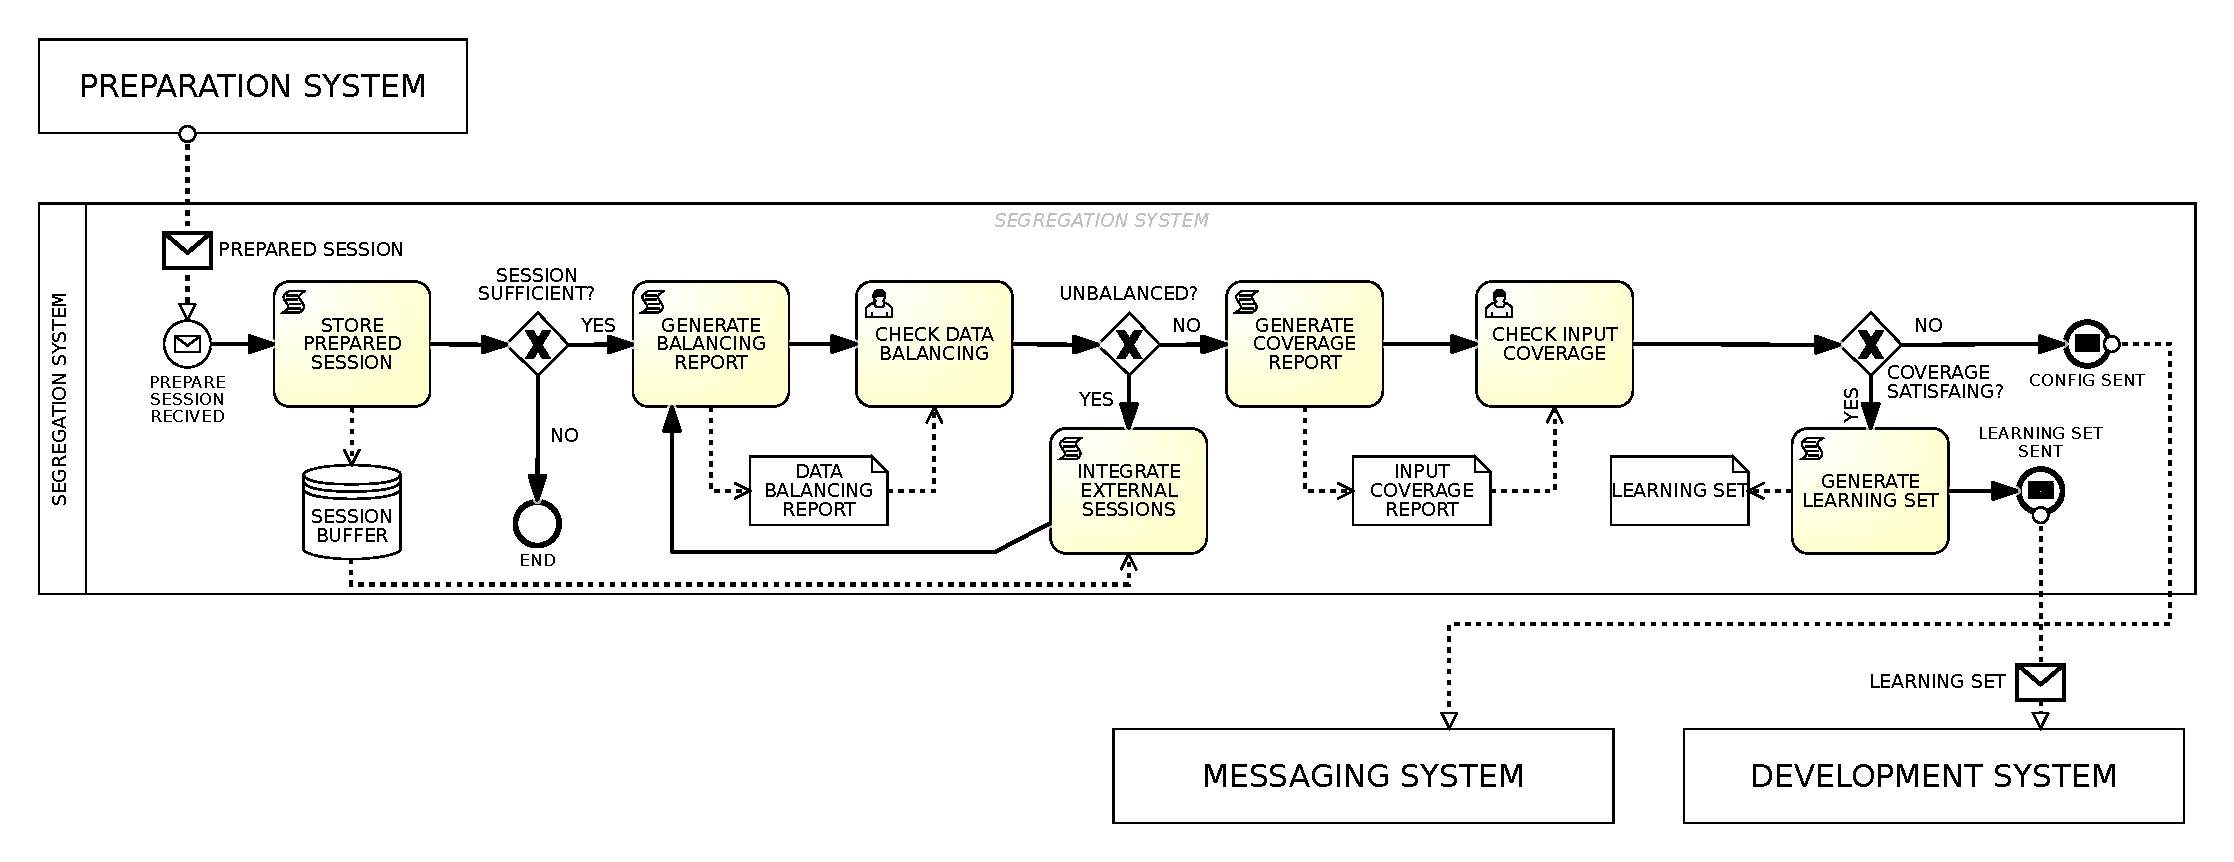
\includegraphics[width=1\textwidth]{figures/TO-BE Business Diagram - Generate Learning Sets.pdf}
    \caption{Change to the Generate Learning Sets}
    \label{fig:to_be_generate_learning_sets}
\end{figure}

We modified the workflow in such a way that our saved previous sessions
can be reused in the case of unbalanced data, rather than awaiting for the
message system to respond to the issue arisen in the workflow.

This cuts on necessary times to respond to this erroneous situation, as the
system can autonomously respond to the issue, rather than waiting for a human
to intervene, thus improving the system's efficiency and re-use of data.



\subsubsection{Service Level Improvement(s)}
\label{subsec:service_level_improvements}
\ididthis{Francesco Boldrini, Zahra Omrani}

\begin{figure}[H]
    \centering
    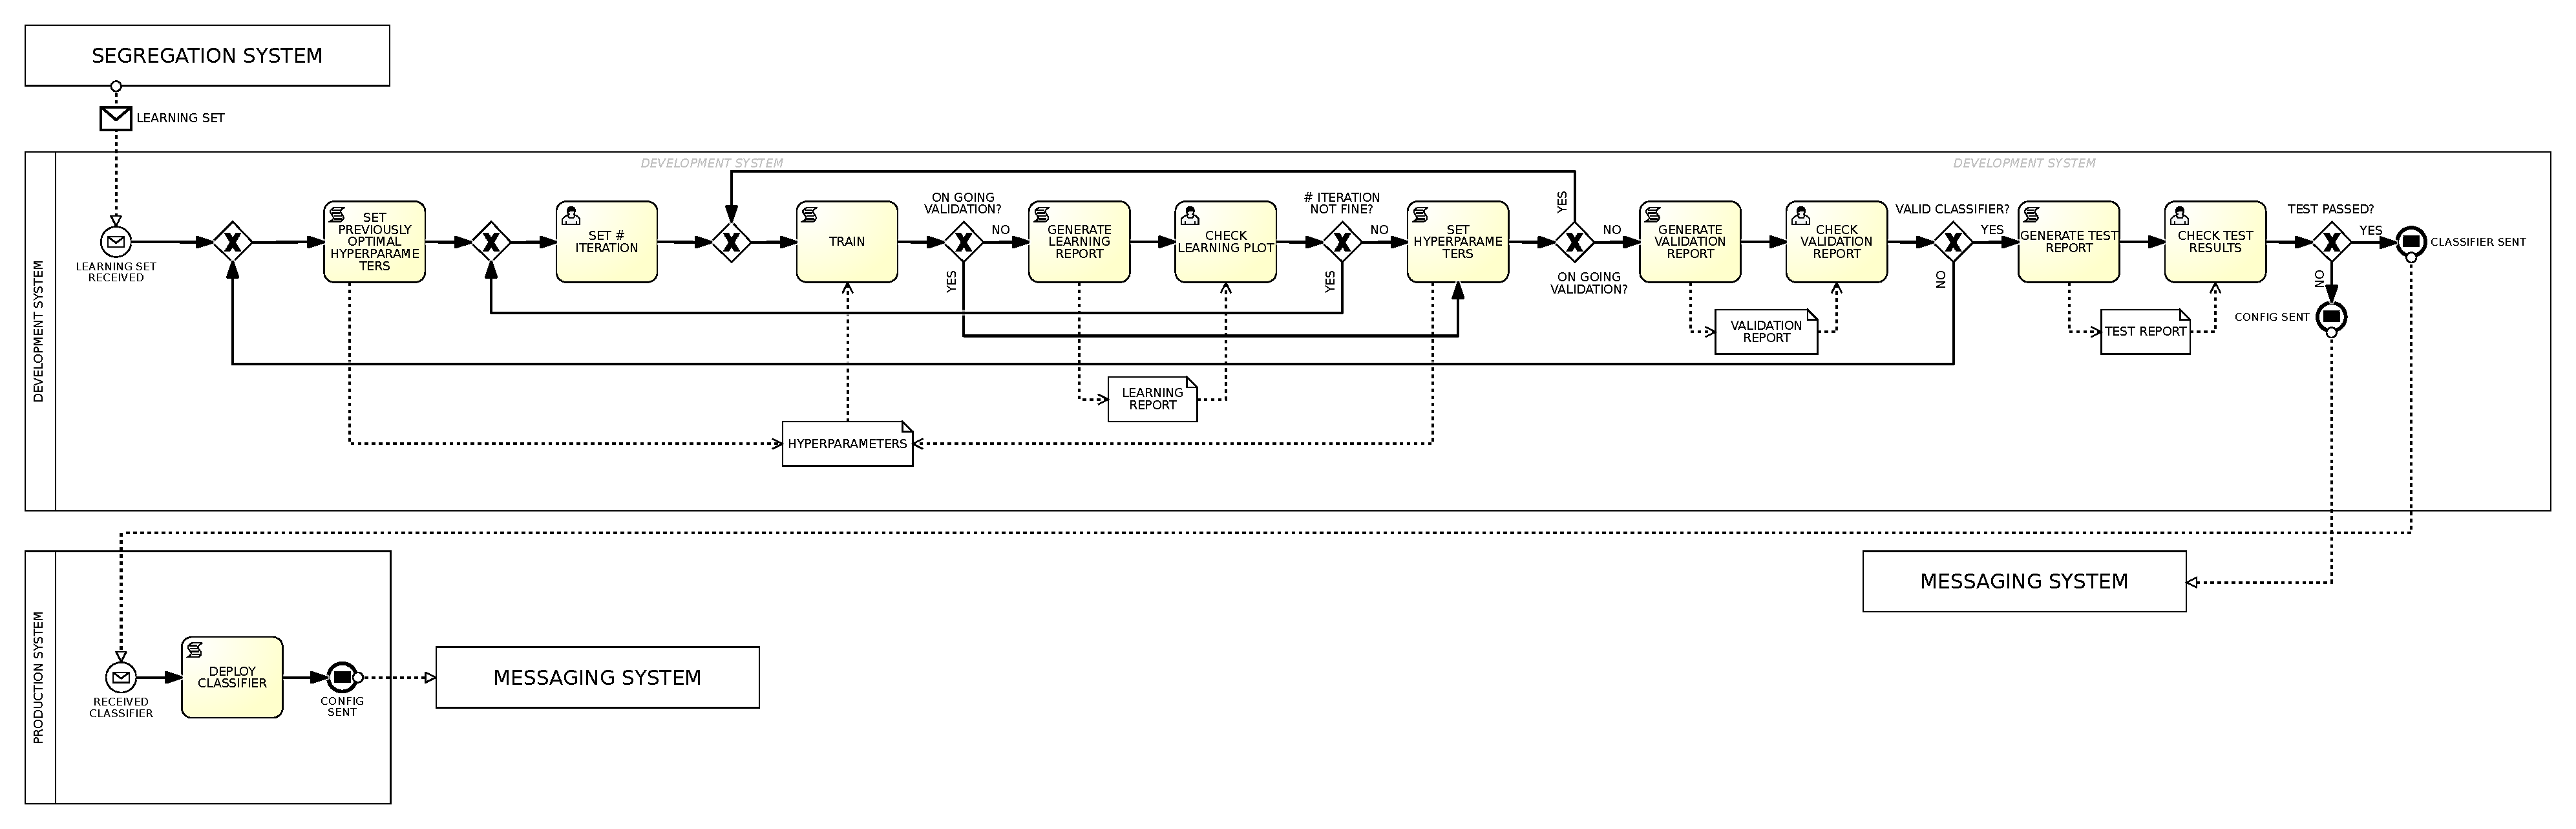
\includegraphics[width=1\textwidth]{figures/TO-BE Business Diagram - Develop Classifier.pdf}
    \caption{Change to the Develop Classifier}
    \label{fig:to_be_develop_classifier}
\end{figure}

The possibility of using hyperparameters from similar trained networks in the same category, rather than starting from scratch, is a great improvement in the service level.

The search for optimized parameters in the network no longer involves brute-forcing the optimization through a grid-search approach but rather re-uses a functioning network's parameters, saving time and computational resources.



\subsubsection{Task Level Improvement(s)}
\label{subsec:task_level_improvements}
\ididthis{Francesco Boldrini, Zahra Omrani}

The task level improvement(s) involve reducing the cognitive effort necessary for the configurations, by starting from default parameters obtained from other similar networks, rather than starting from scratch.

In particular, we removed the need for a grid search in the check validation report, as we no longer need to check amongst the 5 best networks, but simply have to verify that the network respects the overfitting tolerance, as we are using parameters from a similar network in the same category.

\begin{table}[H]
\centering
\begin{tabularx}{\textwidth}{|X|c|c|c|c|}
\hline
\textbf{Step} & \textbf{O} & \textbf{CL} & \textbf{S} & \textbf{SC} \\
\hline
\textbf{1} \textbf{ACTOR} opens "Check validation report" form. & 1 & 1 & 2.5 & 2.5 \\
\hline
\textbf{2} \textbf{SYSTEM} shows the model trained on optimal parameters & & & & \\
\hline
\textbf{3} \textbf{ACTOR} calculates model Validation Loss minus the Training Loss & 1 & 3 & 2.5 & 7.5 \\
\hline
\textbf{4.1} \textbf{IF 3} is less than the Overfitting Tolerance & 0.95 & 3 & 2.5 & 7.125 \\
\hline
\textbf{3.1.1} \textbf{THEN} \textbf{ACTOR} Confirms the selected model. & 0.95 & 3 & 2.5 & 7.125 \\
\hline
\textbf{3.2} \textbf{ELSE} \textbf{ACTOR} Rejects the selected model. & 0.05 & 3 & 2.5 & 0.375 \\
\hline
\textbf{6} \textbf{SYSTEM} shows a confirmation dialog. & & & & \\
\hline
\textbf{7} \textbf{ACTOR} closes the form. & 1 & 1 & 2.5 & 2.5 \\
\hline
\multicolumn{4}{|r|}{Human task cost} & 27.125 $ < $ 175.5 \\
\hline
\end{tabularx}
\caption{Detailed use case for "Check validation report" task\\ 
O - Occurrence, CL - Cognitive Level, S - Normalized Salary, SC - Step Cost}
\label{table:to_be_check_validation_report}
\end{table}

Furthermore, by using suggested parameters in the configuration phase, we can reduce the cognitive level necessary for the configurations to 2 from 4, by starting from default parameters obtained from other similar networks, rather than needing extensive evaluations (level 4 cognitive level) to find the optimal parameters.

\begin{table}[H]
\centering
\begin{tabularx}{\textwidth}{|X|c|c|c|c|}
\hline
\textbf{Step} & \textbf{O} & \textbf{CL} & \textbf{S} & \textbf{SC} \\
\hline
\textbf{1} \textbf{ACTOR} opens the "Configure Preparation System" form. & 1 & 1 & 2.50 & 2.50 \\
\hline
\textbf{2} \textbf{SYSTEM} displays the current configuration. &  &  &  &  \\
\hline
\textbf{3} \textbf{ACTOR} sets the \texttt{alpha\_max}. & 1 & 2 & 2.50 & 5 \\
\hline
\textbf{4} \textbf{ACTOR} sets the \texttt{alpha\_min}. & 1 & 2 & 2.50 & 5 \\
\hline
\textbf{5} \textbf{ACTOR} sets the \texttt{beta\_max}. & 1 & 2 & 2.50 & 5 \\
\hline
\textbf{6} \textbf{ACTOR} sets the \texttt{beta\_min}. & 1 & 2 & 2.50 & 5 \\
\hline
\textbf{7} \textbf{ACTOR} sets the \texttt{theta\_max}. & 1 & 2 & 2.50 & 5 \\
\hline
\textbf{8} \textbf{ACTOR} sets the \texttt{theta\_min}. & 1 & 2 & 2.50 & 5 \\
\hline
\textbf{9} \textbf{ACTOR} sets the \texttt{delta\_max}. & 1 & 2 & 2.50 & 5 \\
\hline
\textbf{10} \textbf{ACTOR} sets the \texttt{delta\_min}. & 1 & 2 & 2.50 & 5 \\
\hline
\textbf{11} \textbf{ACTOR} sets the \texttt{production\_sys\_addr}. & 1 & 1 & 2.50 & 2.50 \\
\hline
\textbf{12} \textbf{ACTOR} sets the \texttt{segregation\_sys\_addr}. & 1 & 1 & 2.50 & 2.50 \\
\hline
\textbf{13} \textbf{ACTOR} selects the \texttt{phase} from the dropdown (\texttt{inference}, \texttt{develop}, \texttt{evaluation}). & 1 & 1 & 2.50 & 2.50 \\
\hline
\textbf{14} \textbf{SYSTEM} {IF} the configuration is correct and properly formatted: &  &  &  &  \\
\hline
\textbf{14.1} \textbf{SYSTEM} displays a confirmation message. & & & &  \\
\hline
\textbf{14.2} \textbf{ELSE} (if the configuration is incorrect): & & &  &  \\
\hline
\textbf{14.2.1} \textbf{SYSTEM} displays an error message and aborts the process. &  &  &  &  \\
\hline
\textbf{15} \textbf{ACTOR} saves the form. & 1 & 1 & 2.50 & 2.50 \\
\hline
\multicolumn{4}{|r|}{\textbf{Human task cost}} & 52.5 $ < $ 92.5 \\
\hline
\end{tabularx}
\caption{TO-BE detailed use case for "Configure Preparation System" task}
\label{table:to_be_configure_preparation_system}
\end{table}


\subsection{TO-BE Simulation}
\label{sec:to_be_simulation}
\ididthis{Francesco Boldrini, Zahra Omrani}




\begin{figure}[H]
    \centering
    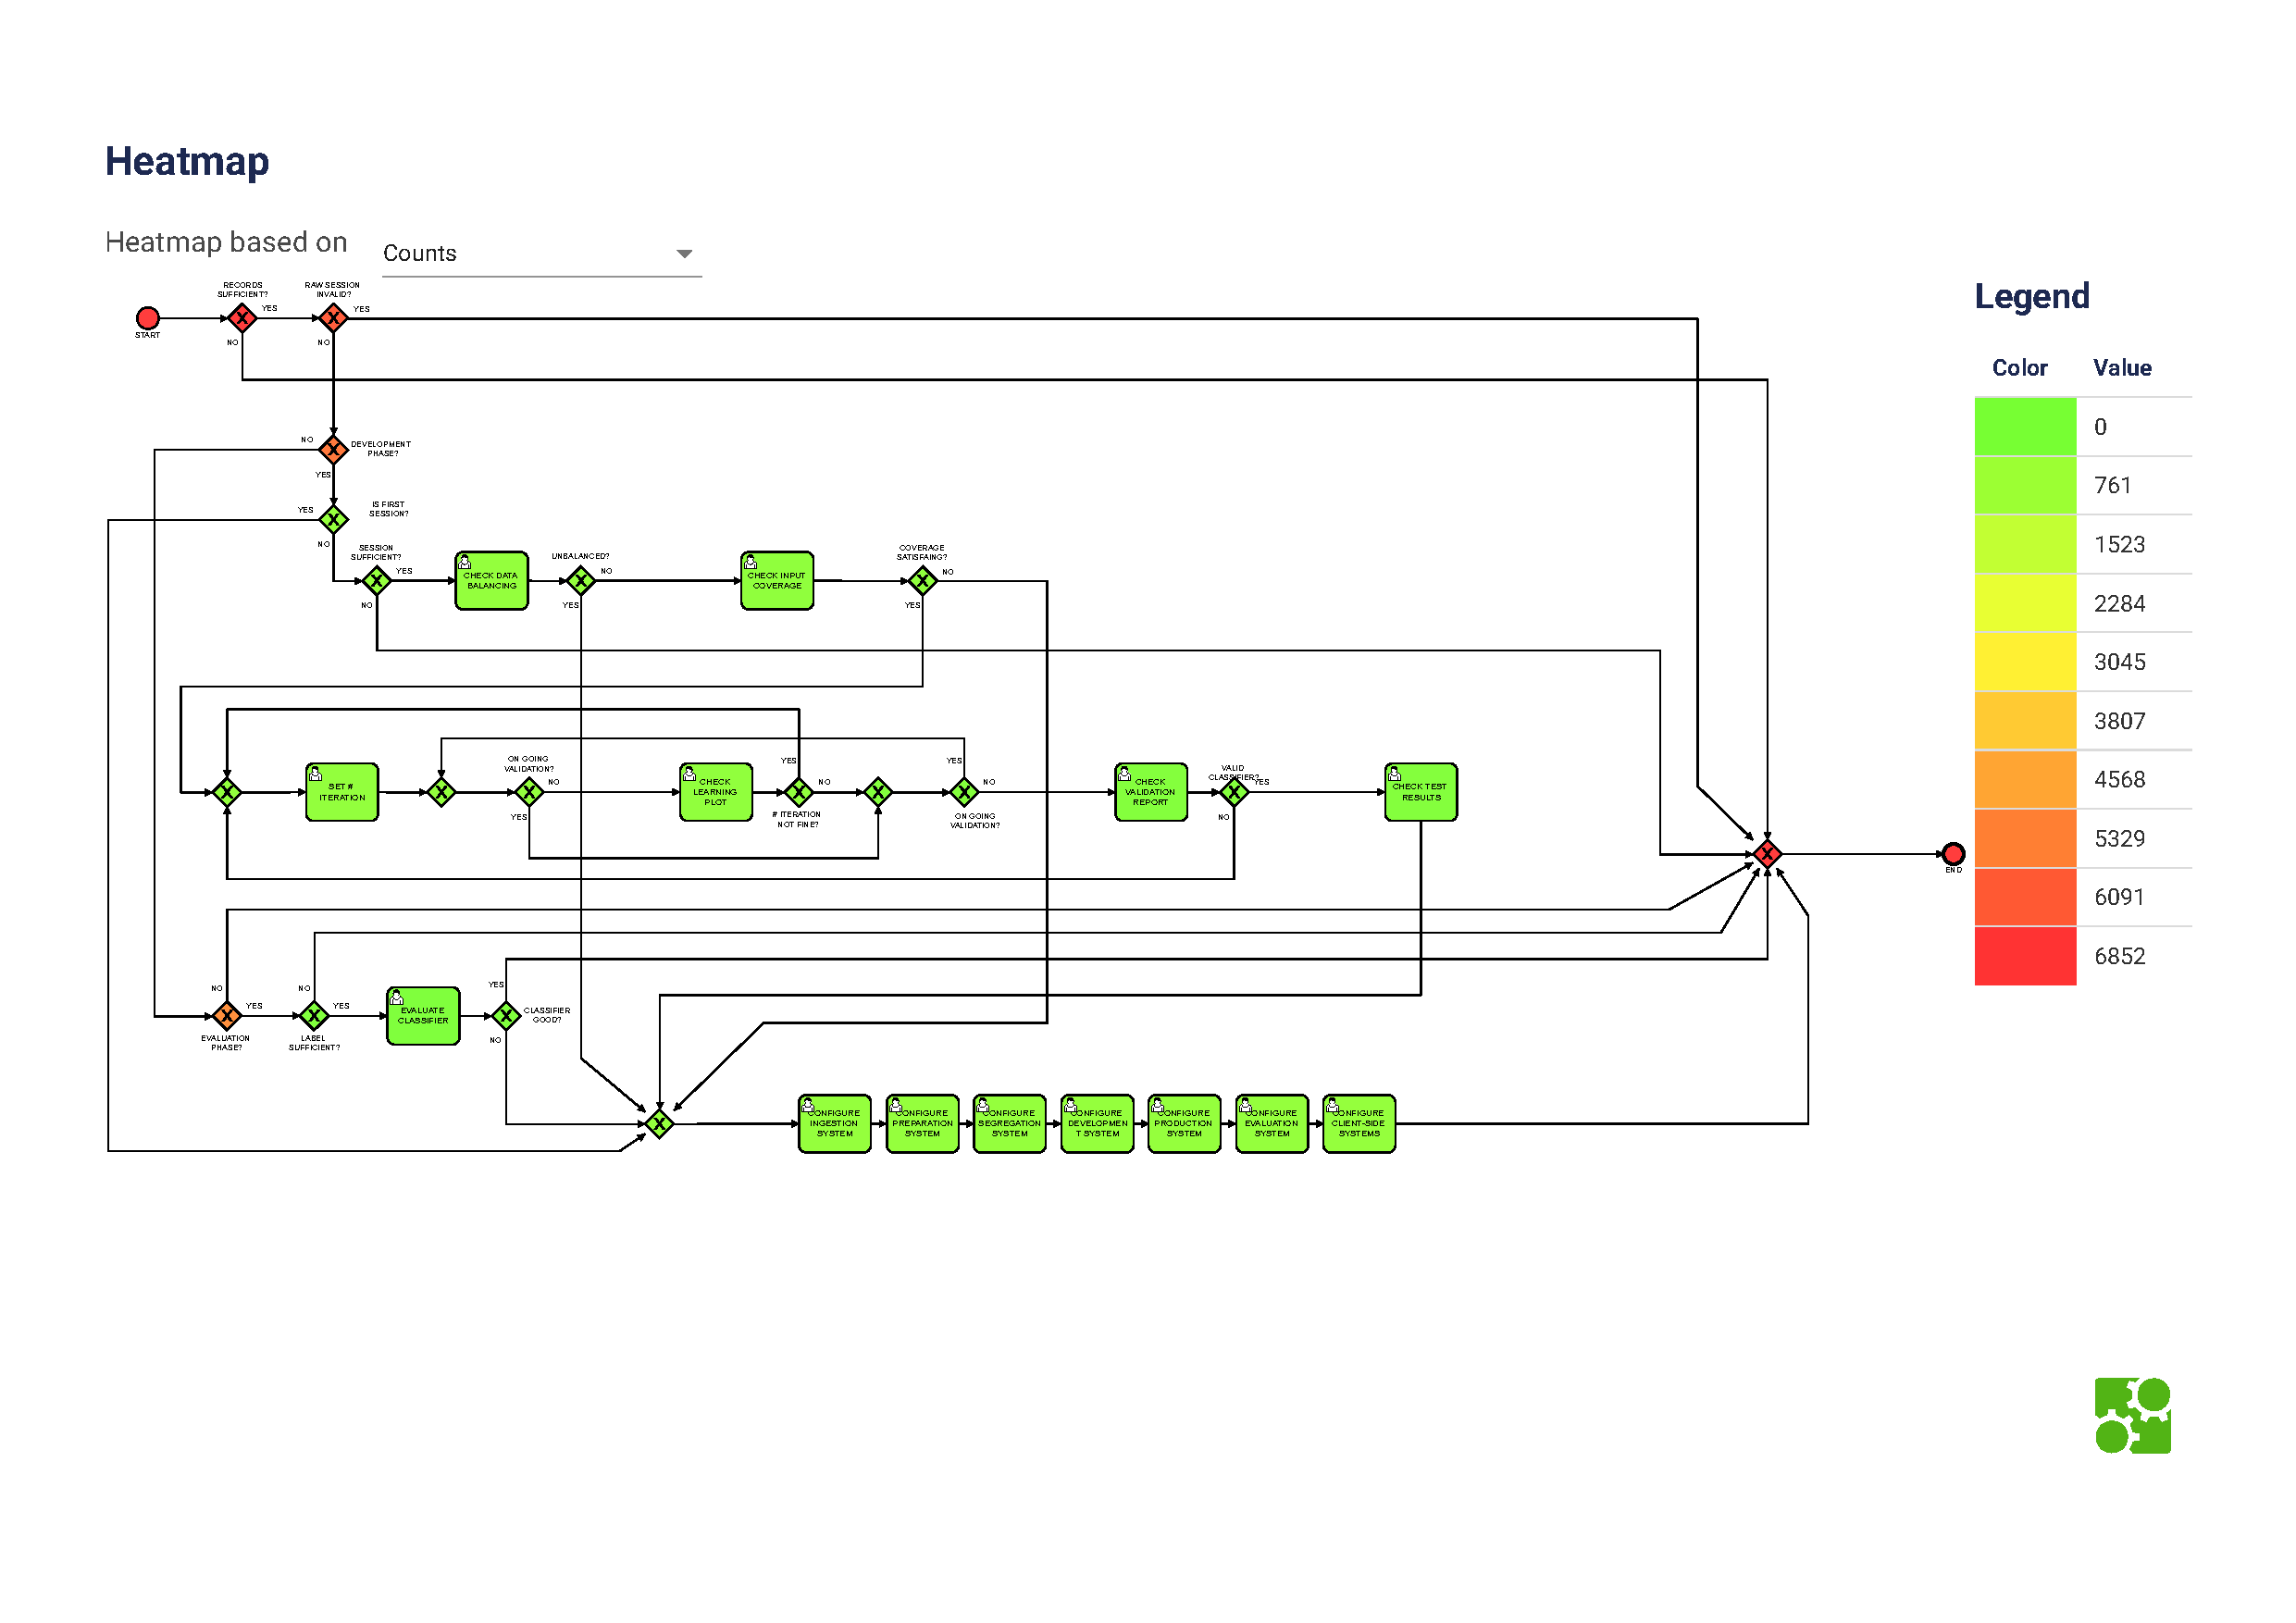
\includegraphics[width=0.87\textwidth]{figures/TO-BE heatmap_counts.pdf}
    \caption{TO-BE Heatmap of the counts of the parameters}
    \label{fig:to_be_heatmap_counts}
\end{figure}

\begin{figure}[H]
    \centering
    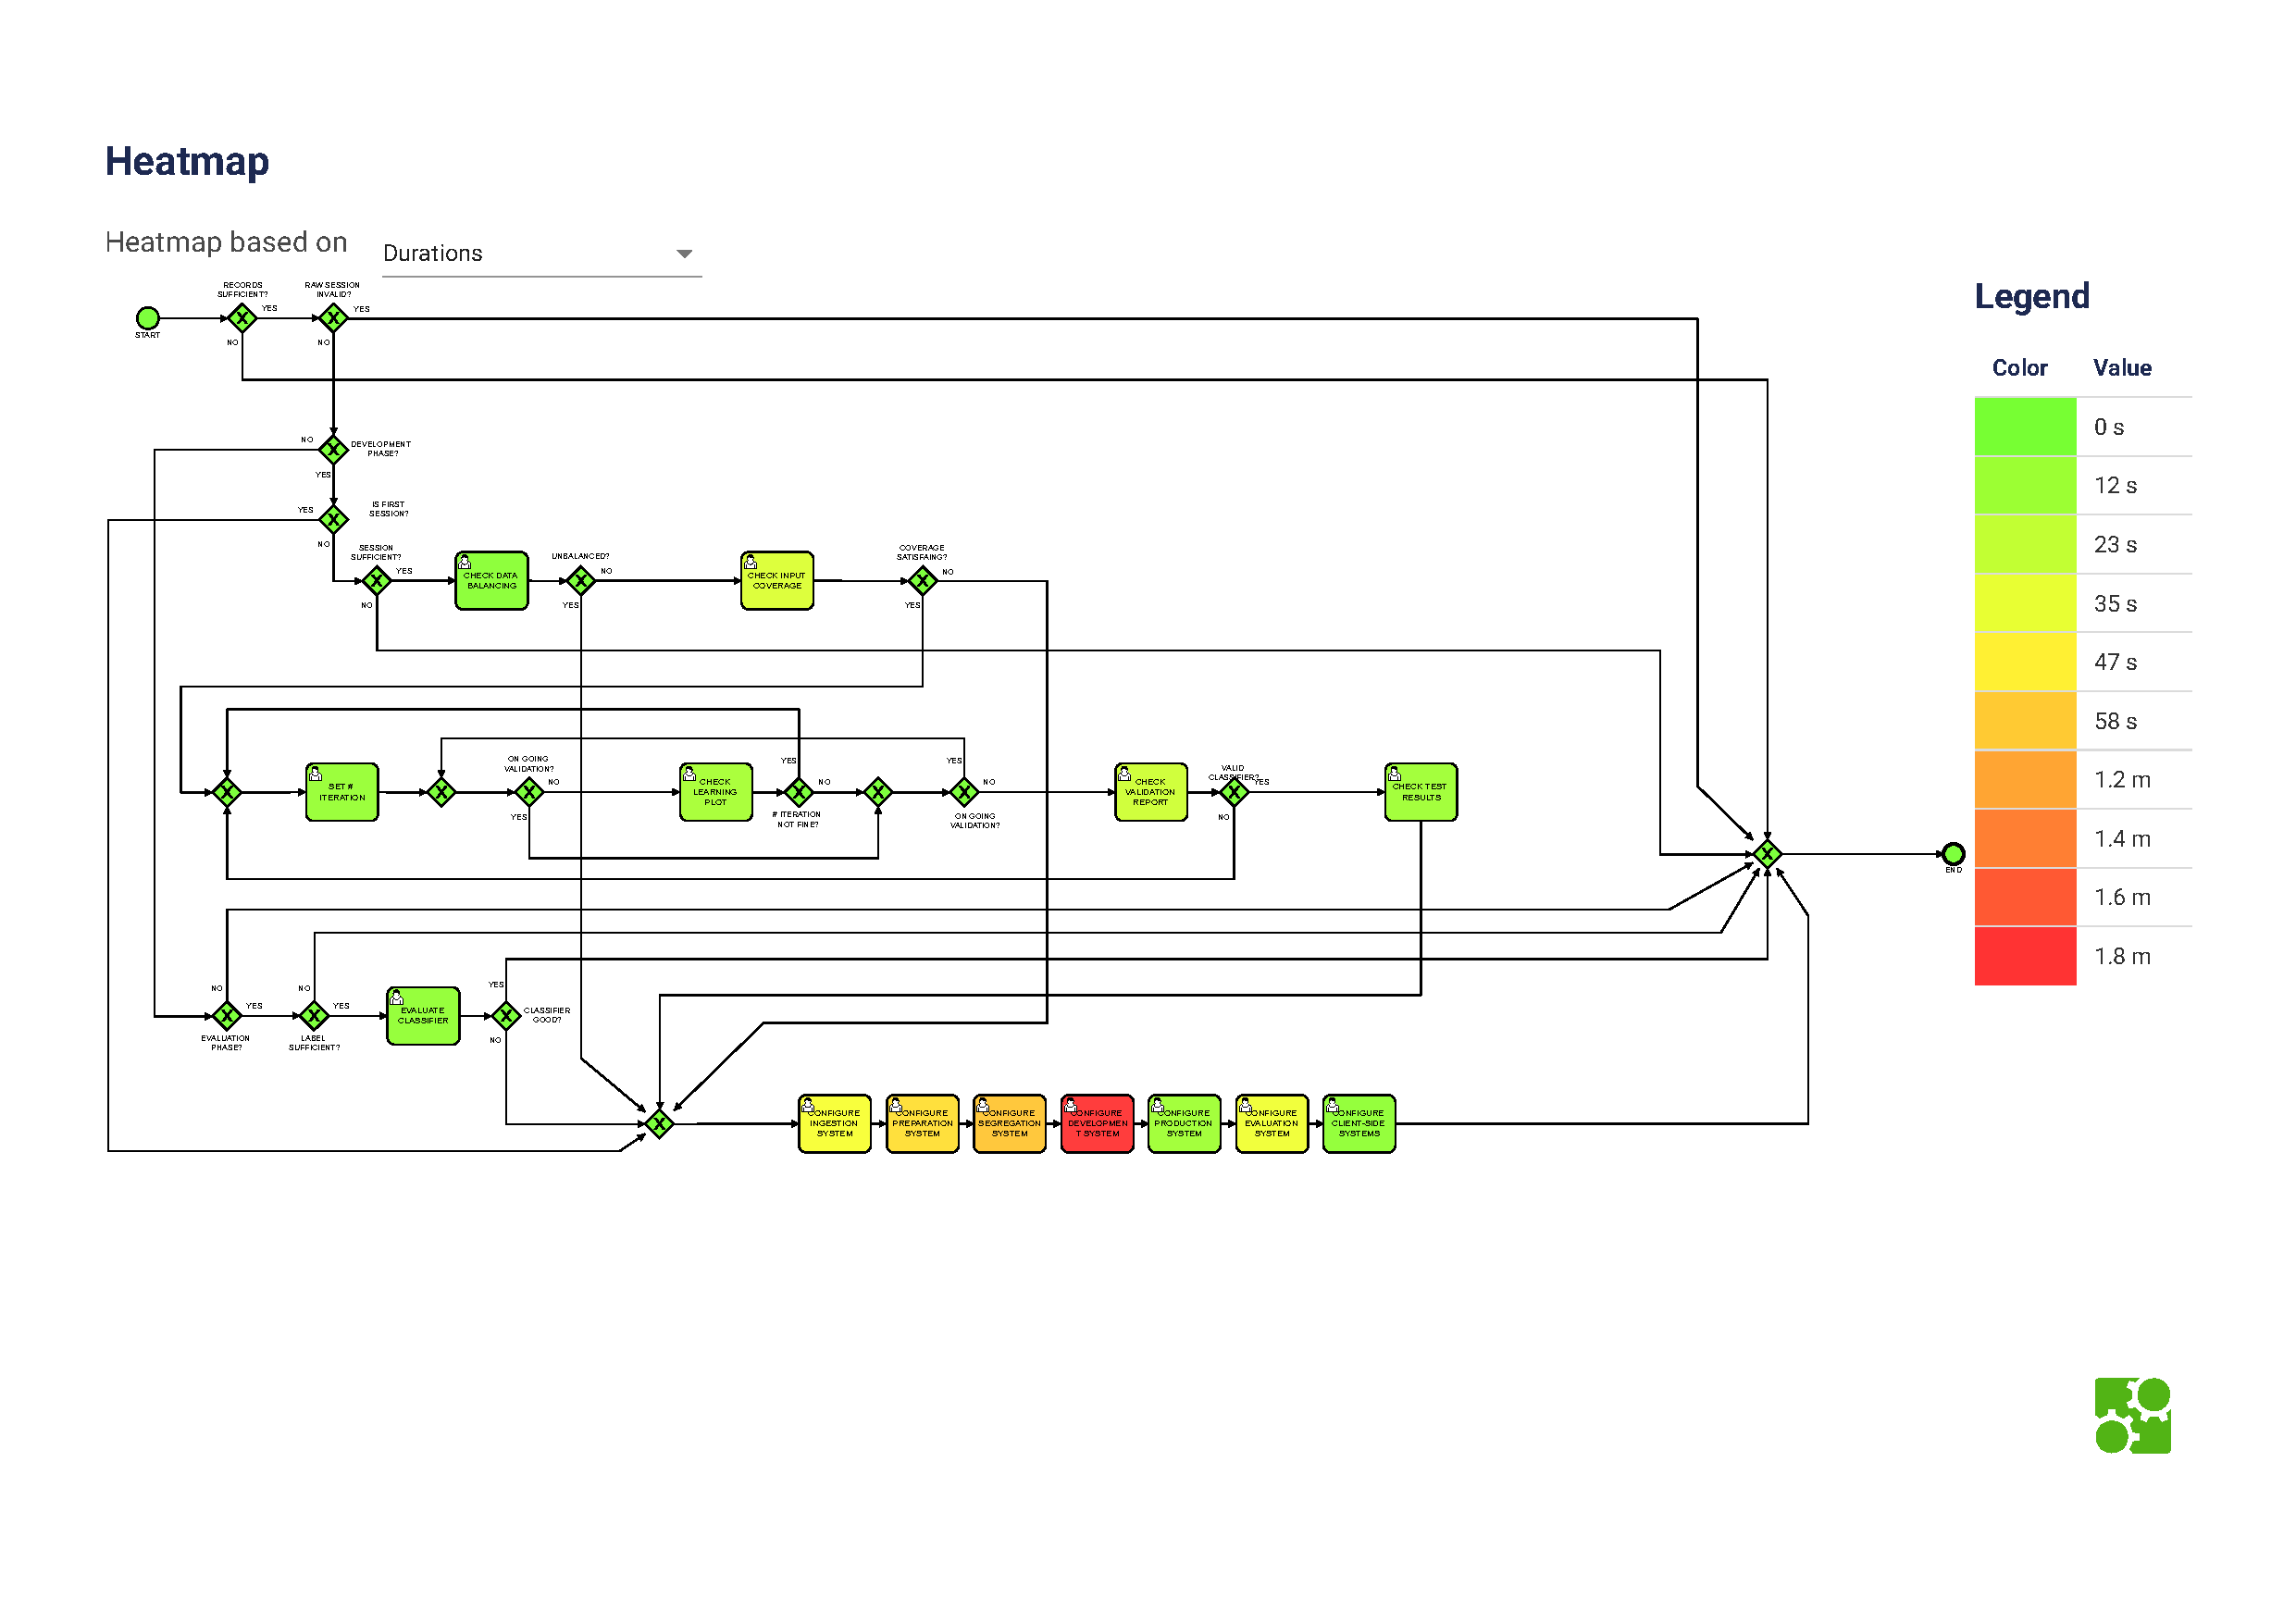
\includegraphics[width=0.87\textwidth]{figures/TO-BE heatmap_durations.pdf}
    \caption{TO-BE Heatmap of the time spent in each passage [Durations]}
    \label{fig:to_be_heatmap_durations}
\end{figure}

\begin{figure}[H]
    \centering
    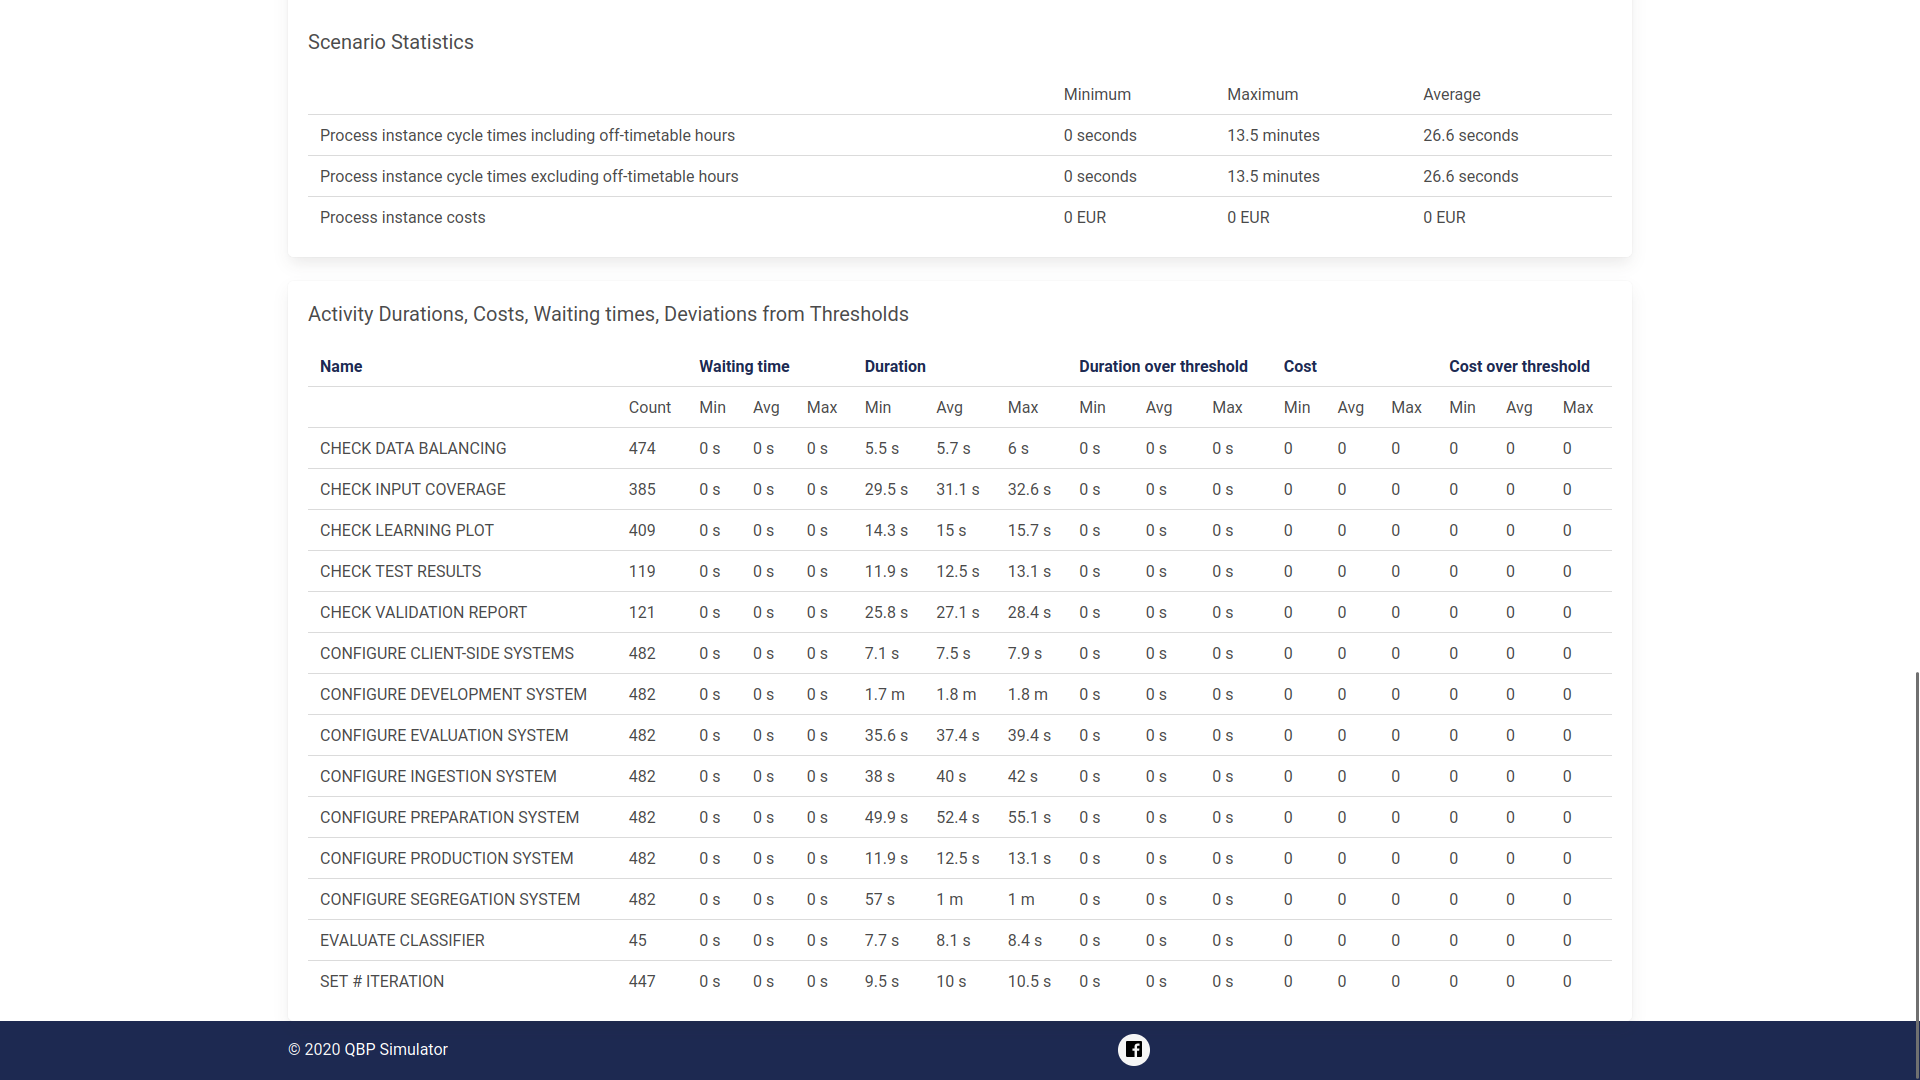
\includegraphics[width=1\textwidth]{figures/TO-BE Simulation Results.png}
    \caption{TO-BE Simulation Results}
    \label{fig:to_be_simulation_results}
\end{figure}

\begin{figure}[H]
    \centering
    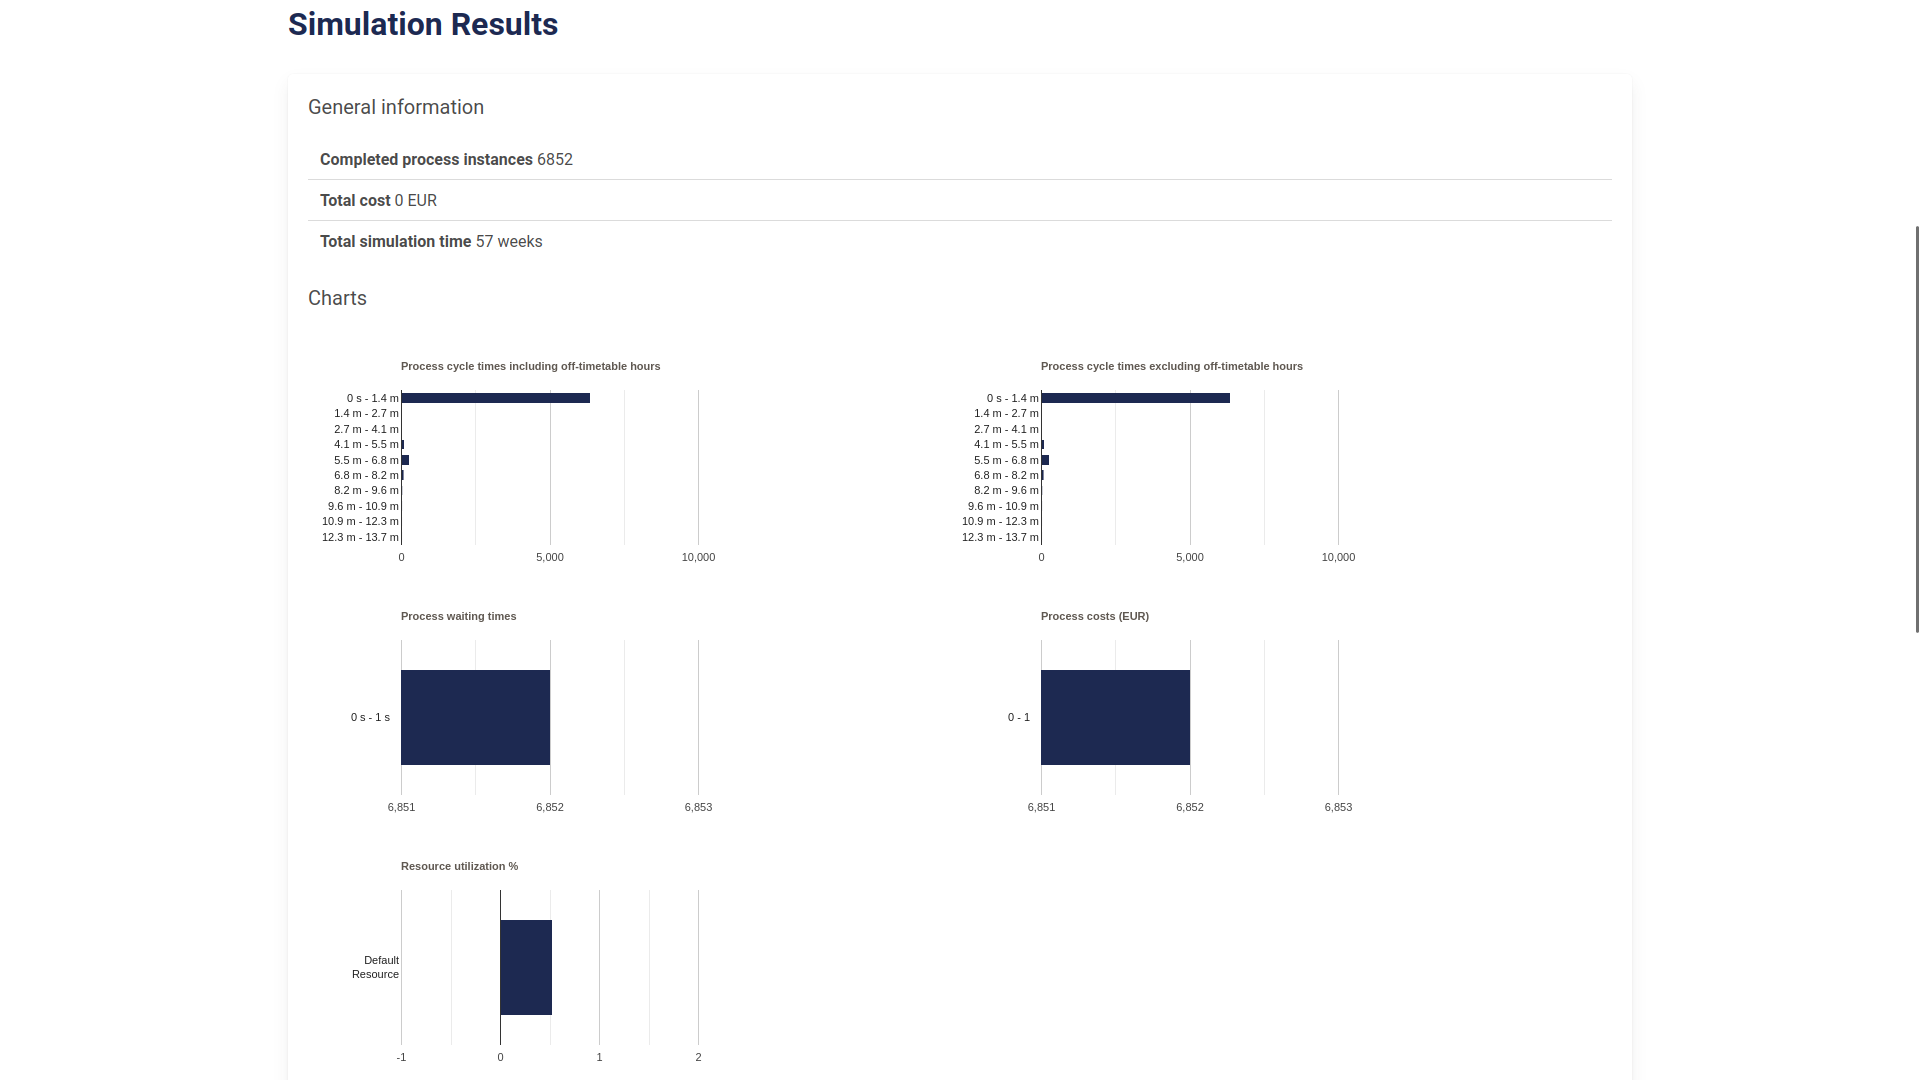
\includegraphics[width=1\textwidth]{figures/TO-BE Scenario Statistics.png}
    \caption{TO-BE Scenario Statistics}
    \label{fig:to_be_scenario_Statistics}
\end{figure}

